\section{Введение}

Гипероктаэдральные или кубические комбинаторные виды --- развите идеи комбинаторных типов (species).
Мы будем обозначать их h-species для краткости.
TODO:добавить введение (видимо взять часть из Bergeron)

План:
Изложить теорию для species, параллельно строить ее для h-species

species --- сложение умножение --- аналитический функтор --- композиция
аналитических функторов --- композиция species --- декатегорификация
аналитического функтора --- примеры

\subsection{Комбинаторные виды}
Комбинаторные виды (\emph{species}) были введены Джоялем в [ref, ref, ref].
Они, в некоторой степени, являются развитием идеи производящих функций.
О комбинаторных видах можно говорить на нескольких языках: категорном,
комбинаторном и на языке теории представлений. Последний наиболее часто
встречается в литературе, хотя автору он кажется наимение выразительным.
Во введении будет изложено начало теории комбинаторных видов.
\subsubsection{Определение}
Рассмотрим категорию $\mathcal B$ --- подкатегорию конечных множеств с
морфизмами --- биекциями конечных множеств. Это подкатегория в $Set$. Функтор
$F:\mathcal B \rightarrow Set$ --- это комбинаторный вид. То есть вид, это
сопоставление каждому числу $n \in \mathbb N$ множества с действием группы
$S_n$. Комбинаторная интерпретация: множеству точек сопоставляются
структуры на точках, а действие $S_n$ ествественно возникает из перестановок
исходных точек. Например, вид $\mathbb E$ --- структура множеста. Он
сопоставляет набору точек одно множество, состоящие из этих точек. Все элементы $S_n$
переходят в тождественное отображение. Другой пример $\mathbb C$ --- циклический
порядок. Сопоставляет набору из $n$ точек $(n-1)!$ возможных циклических
порядков на них. Линейный порядок $\mathbb L$ сопоставляет $n!$ линейных
порядков. На картинке \ref{pic-3-rooted-trees} изображен вид <<корневые
деревья с 3 вершинами>> (без какого-либо порядка на потомках).

\begin{center}
\label{pic-3-rooted-trees}
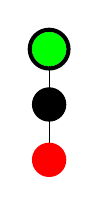
\begin{tikzpicture}
\draw (0pt, 0pt) -- (0pt, -20pt);
\draw (0pt, -20pt) -- (0pt, -40pt);
\draw[color=green, fill] (0pt,0pt) circle (6pt);
\draw[color=black, line width=1.5pt] (0pt,0pt) circle (7pt);
\draw[color=black, fill] (0pt, -20pt) circle (6pt);
\draw[color=red, fill] (0pt, -40pt) circle (6pt);
\end{tikzpicture}
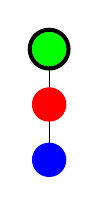
\begin{tikzpicture}
\draw (0pt, 0pt) -- (0pt, -20pt);
\draw (0pt, -20pt) -- (0pt, -40pt);
\draw[color=green, fill] (0pt,0pt) circle (6pt);
\draw[color=black, line width=1.5pt] (0pt,0pt) circle (7pt);
\draw[color=red, fill] (0pt, -20pt) circle (6pt);
\draw[color=blue, fill] (0pt, -40pt) circle (6pt);
\end{tikzpicture}
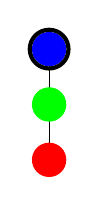
\begin{tikzpicture}
\draw (0pt, 0pt) -- (0pt, -20pt);
\draw (0pt, -20pt) -- (0pt, -40pt);
\draw[color=blue, fill] (0pt,0pt) circle (6pt);
\draw[color=black, line width=1.5pt] (0pt,0pt) circle (7pt);
\draw[color=green, fill] (0pt, -20pt) circle (6pt);
\draw[color=red, fill] (0pt, -40pt) circle (6pt);
\end{tikzpicture}
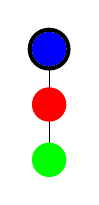
\begin{tikzpicture}
\draw (0pt, 0pt) -- (0pt, -20pt);
\draw (0pt, -20pt) -- (0pt, -40pt);
\draw[color=blue, fill] (0pt,0pt) circle (6pt);
\draw[color=black, line width=1.5pt] (0pt,0pt) circle (7pt);
\draw[color=red, fill] (0pt, -20pt) circle (6pt);
\draw[color=green, fill] (0pt, -40pt) circle (6pt);
\end{tikzpicture}
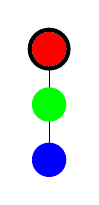
\begin{tikzpicture}
\draw (0pt, 0pt) -- (0pt, -20pt);
\draw (0pt, -20pt) -- (0pt, -40pt);
\draw[color=red, fill] (0pt,0pt) circle (6pt);
\draw[color=black, line width=1.5pt] (0pt,0pt) circle (7pt);
\draw[color=green, fill] (0pt, -20pt) circle (6pt);
\draw[color=blue, fill] (0pt, -40pt) circle (6pt);
\end{tikzpicture}
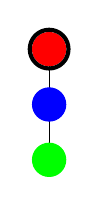
\begin{tikzpicture}
\draw (0pt, 0pt) -- (0pt, -20pt);
\draw (0pt, -20pt) -- (0pt, -40pt);
\draw[color=red, fill] (0pt,0pt) circle (6pt);
\draw[color=black, line width=1.5pt] (0pt,0pt) circle (7pt);
\draw[color=blue, fill] (0pt, -20pt) circle (6pt);
\draw[color=green, fill] (0pt, -40pt) circle (6pt);
\end{tikzpicture}
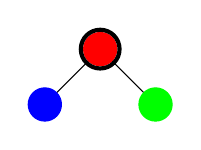
\begin{tikzpicture}
\draw (0pt, 0pt) -- (-20pt, -20pt);
\draw (0pt, 0pt) -- (20pt, -20pt);
\draw[color=red, fill] (0pt,0pt) circle (6pt);
\draw[color=black, line width=1.5pt] (0pt,0pt) circle (7pt);
\draw[color=blue, fill] (-20pt, -20pt) circle (6pt);
\draw[color=green, fill] (20pt, -20pt) circle (6pt);
\end{tikzpicture}
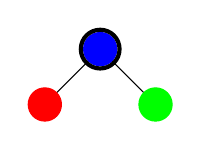
\begin{tikzpicture}
\draw (0pt, 0pt) -- (-20pt, -20pt);
\draw (0pt, 0pt) -- (20pt, -20pt);
\draw[color=blue, fill] (0pt,0pt) circle (6pt);
\draw[color=black, line width=1.5pt] (0pt,0pt) circle (7pt);
\draw[color=red, fill] (-20pt, -20pt) circle (6pt);
\draw[color=green, fill] (20pt, -20pt) circle (6pt);
\end{tikzpicture}
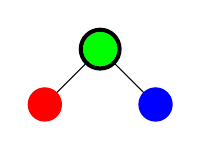
\begin{tikzpicture}
\draw (0pt, 0pt) -- (-20pt, -20pt);
\draw (0pt, 0pt) -- (20pt, -20pt);
\draw[color=green, fill] (0pt,0pt) circle (6pt);
\draw[color=black, line width=1.5pt] (0pt,0pt) circle (7pt);
\draw[color=red, fill] (-20pt, -20pt) circle (6pt);
\draw[color=blue, fill] (20pt, -20pt) circle (6pt);
\end{tikzpicture}
\end{center}

Можно рассмотреть функтор $I:Set \rightarrow Vec$, который сопоставляет множеству
векторное пространство со свободным базисом из этого множества. Тогда $F \circ
I: \mathcal B \rightarrow Vec$, получается для каждого $n$
перестановочное представление группы $S_n$. При таком подходе, характер этого
представления $\chi(\sigma)$, это количество структур, неподвижных относительно $\sigma \in S_n$.


ТЕОРЕМА: композиции аналитически функторов соответсвует плетизм цикленных
индексов.
